\mysubsubsection{Layered depthmap estimation}

\noindent We have used ``ours\_1'' data in~\cite{layered_depthmap} for
the experiments. Figure.~\ref{fig:layered_depthmap_convergence} shows that
Fusion Move, Parallel Fusion Move and SF-MF all got stuck in local
minima, which is due to the lack of multi-way fusion.  Layered depthmap
estimation is a challenging problem with very large solution space. The
binary fusion of solution proposals is too restrictive to make any
improvements.  This coincides with the observation in
\cite{layered_depthmap} that binary fusion of proposal solutions is not
as powerful as their subspace fusion which is a special form of
multi-way fusion here. Lastly, solution sharing also plays an important
role for this challenging problem, as SF performs much better than
SF-SS.

\begin{figure}[!h]
  \centering
  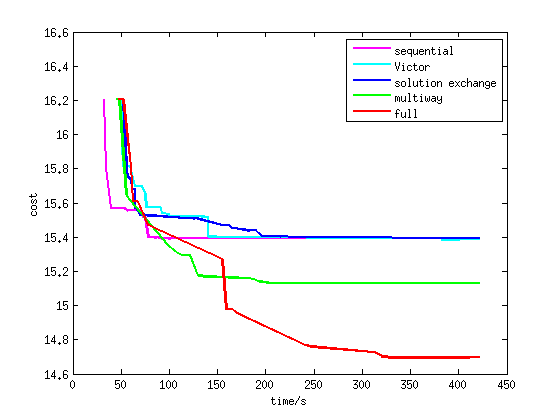
\includegraphics[width=0.8\columnwidth]{figure/layered_depthmap_convergence.png}
  \caption{Energy plots for the layered depthmap estimation
    problem. Both the multi-way fusion and the solution sharing are important
    for this challenging problem.}\label{fig:layered_depthmap_convergence}
\end{figure}

\begin{figure}[!h]
  \centering
  \begin{subfigure}[b]{0.49\columnwidth}
    \centering
    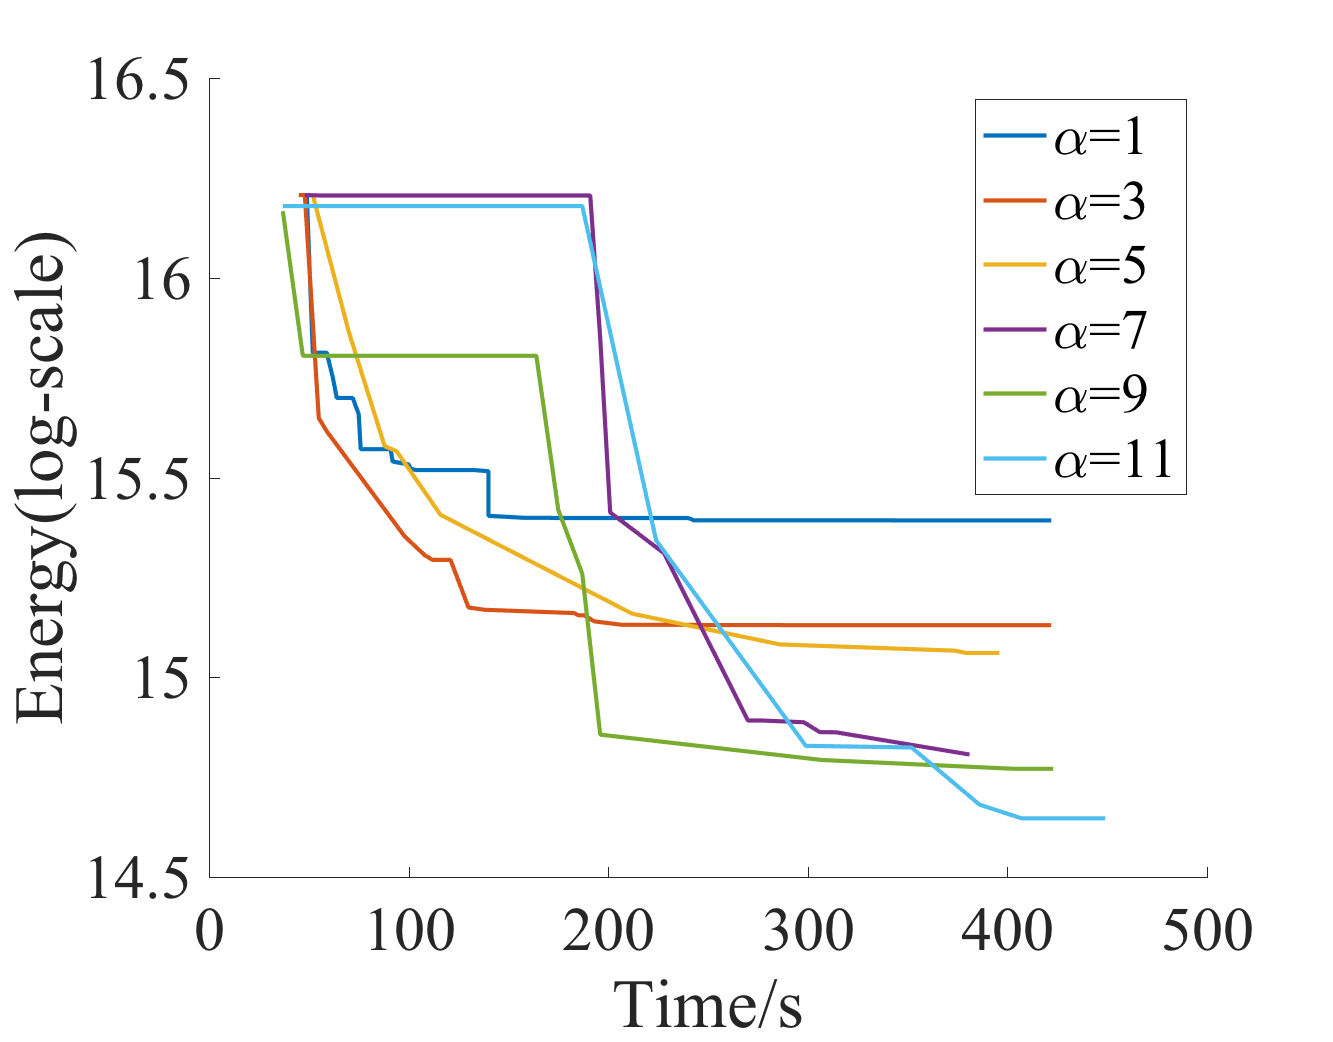
\includegraphics[width=\columnwidth]{figure/layered_depthmap_by_alpha.png}
  \end{subfigure}  
  \begin{subfigure}[b]{0.49\columnwidth}
    \centering
    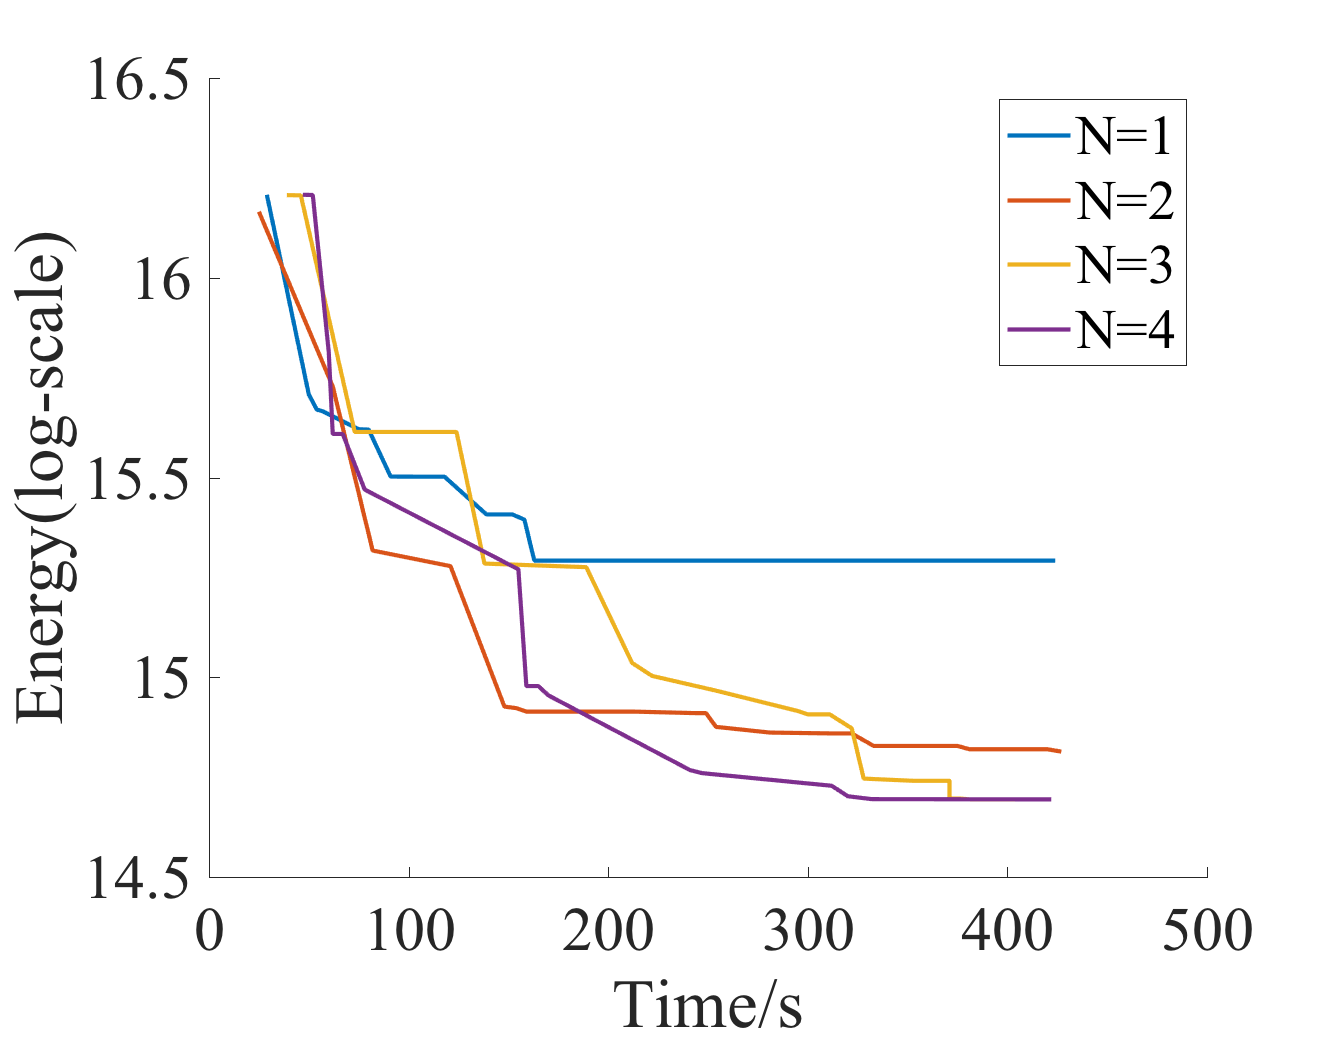
\includegraphics[width=\columnwidth]{figure/layered_depthmap_by_N.png}
  \end{subfigure}
  \caption{Left: Energy plots for layered depthmap estimation with varying
    $\alpha$. Right: Energy plots for layered depthmap estimation with varying number of threads N.}
  \label{fig:layered_depthmap_configuration}
\end{figure}


%
% From the plot, we can see that, Fusion Move, Parallel Fusion Move, and
%SF-MF all stalk at a high energy state.
To further study the effects of multi-way fusion, we have varied the
value of $\alpha$ which controls the number of solution proposals to be
fused in SF-SS model (See
Fig.~\ref{fig:layered_depthmap_configuration}(left)). Note that we have used SF-SS
instead of SF to disable solution sharing and better observe the effects
of multi-way fusion.
% SF-SS model (disable solution sharing to
%better observe the effect of multi-way fusion) while keeping other
%parameters the same and plot the energy minimization process in figure
It is interesting to see that more multi-way fusion takes longer to
converge, but finds a lower energy state at the end.

Finally, we have examined the role of multi-threading by varying the
number of threads N in our most general model SF (See
Fig.~\ref{fig:layered_depthmap_configuration}(right))~\footnote{While keeping other
parameters the same, we have to change $\beta$ with $N$ because of the
constraint $\beta \leq N-1$. We have always used $\beta = N-1$ in this
experiment.}. More threads lead to faster convergence as expected,
although the rate of speed-up is not proportional to the number of
threads due to the randomness in the proposal generation scheme.
%The plot shows that SF finds low energy faster with more
%threads.
% In Fusion Move like methods, parallelism speeds up convergence
% by exploring solution proposals faster. Due to the inherited randomness
% in the proposal generation scheme, the speed up is often not
% proportional to the number of threads.
%We can see that as the number of
%ways to fuse becomes larger, each fusion step takes longer time, but the
%chance of finding a lower energy state increases.
